\chapter{Introduction}

The last decade has seen massive growth in the field of Autonomous
Driving, primarily due to 
\begin{enumerate*}[label= \alph*)]
    \item proliferation of graphical processing unit(GPU),

    \item several projects like Google(Waymo) \cite{Waymo},
        Berkeley-DeepDrive \cite{Berkeley-DeepDrive},
        Apollo \cite{Apollo}, have made their datasets open-source making it
        easier for people to work on these data and achieve better performance gains. 
\end{enumerate*}



Training a deep neural network(DNN) forms the core of making a car autonomous. 
By using supervised learning, one can achieve reliable results as it gives greater control
at each stage of training. The data-driven approach collects data in advance and labels it
appropriately. It can then be fed to the DNN using supervised
learning algorithms to train the best model possible. 

Ever since the discovery of Alexnet in 2012 \cite{Alexnet2012}, the convolutional neural network(CNN) and
deep learning(DL) are preferred choices to analyse images.  However, it is well known that the camera sensors are susceptible even to a slight change in weather conditions. 
Sensors like radar \cite{Radar}, LIDAR \cite{LIDAR}, ultrasonic\cite{ultrasonic}, depth camera
give additional depth information for obstacle detection. These values then are fused with the camera images to make
data fusion possible. 

Even though there are some public data available, it is still not enough to reliably
train a DNN. Then there is  the cost of building an autonomous car. Fortunately, the last
years have seen growth in reliable simulators which
helped massively to collect data to help explore this field of research.
To name a few simulators that are being actively used -- LGSVL \cite{LGSVL}, Nvidia Drive
\cite{NvidiaSimulator}, Carla \cite{CarlaSimulator}, CarMaker \cite{CarMaker}. 
In this thesis, the LGSVL simulator is used.

The LGSVL simulator allows the use of different sensors with minimal effort. The data
from different sensors are published through websocket. So to capture these data, we
need an interface/protocol which can understand the sent data's message types and enable the
receiving node/programme to store them. However, the data from each sensor arrives at
different rates. Hence it is necessary to collect and synchronise them in the order of their arrival
before storing, to not lose their integrity and thereby prevent corrupting the dataset.
Robotic operating system(ROS) \cite{ROS2} and its functionalities fulfil
this purpose. It allows seamless transfer of simulator's data by subscribing to it in the
form of topics. Then the subscribing node synchronises it as necessary for storage.

So, now the data that resembles real-world is stored locally for later analysis and
research.

\section{Motivation}

Though autonomous driving is one of the favourite research areas in mobility, 
a significant challenge is still the cost associated with integrating all the necessary sensors.  
Representing the environment around the vehicle(ego vehicle) requires information from all in-car sensors. 
The resources demanded to make an optimal decision are also a challenge. The motivation for this thesis is 
to use a simulator, do the required tests and 
determine whether using a simulator does indeed help in perceiving the environment 
and accomplish the goal of driving in the real-world. 

As briefly mentioned, the high cost of associated sensors such as LIDAR
\cite{VergeReportLidar},  has put off many smaller research groups from implementing into their
work. By using a simulator, again at a low cost, we can conduct adequate tests 
on how different constellation of sensors work, how different modalities interact with each other and 
what impact these factors have on the overall performance of the DNN.

Finally, implement an end-to-end system which simulates real-world behaviour which can
then be applied to future research and make it more robust.

\begin{figure}[h]
    \begin{center}
        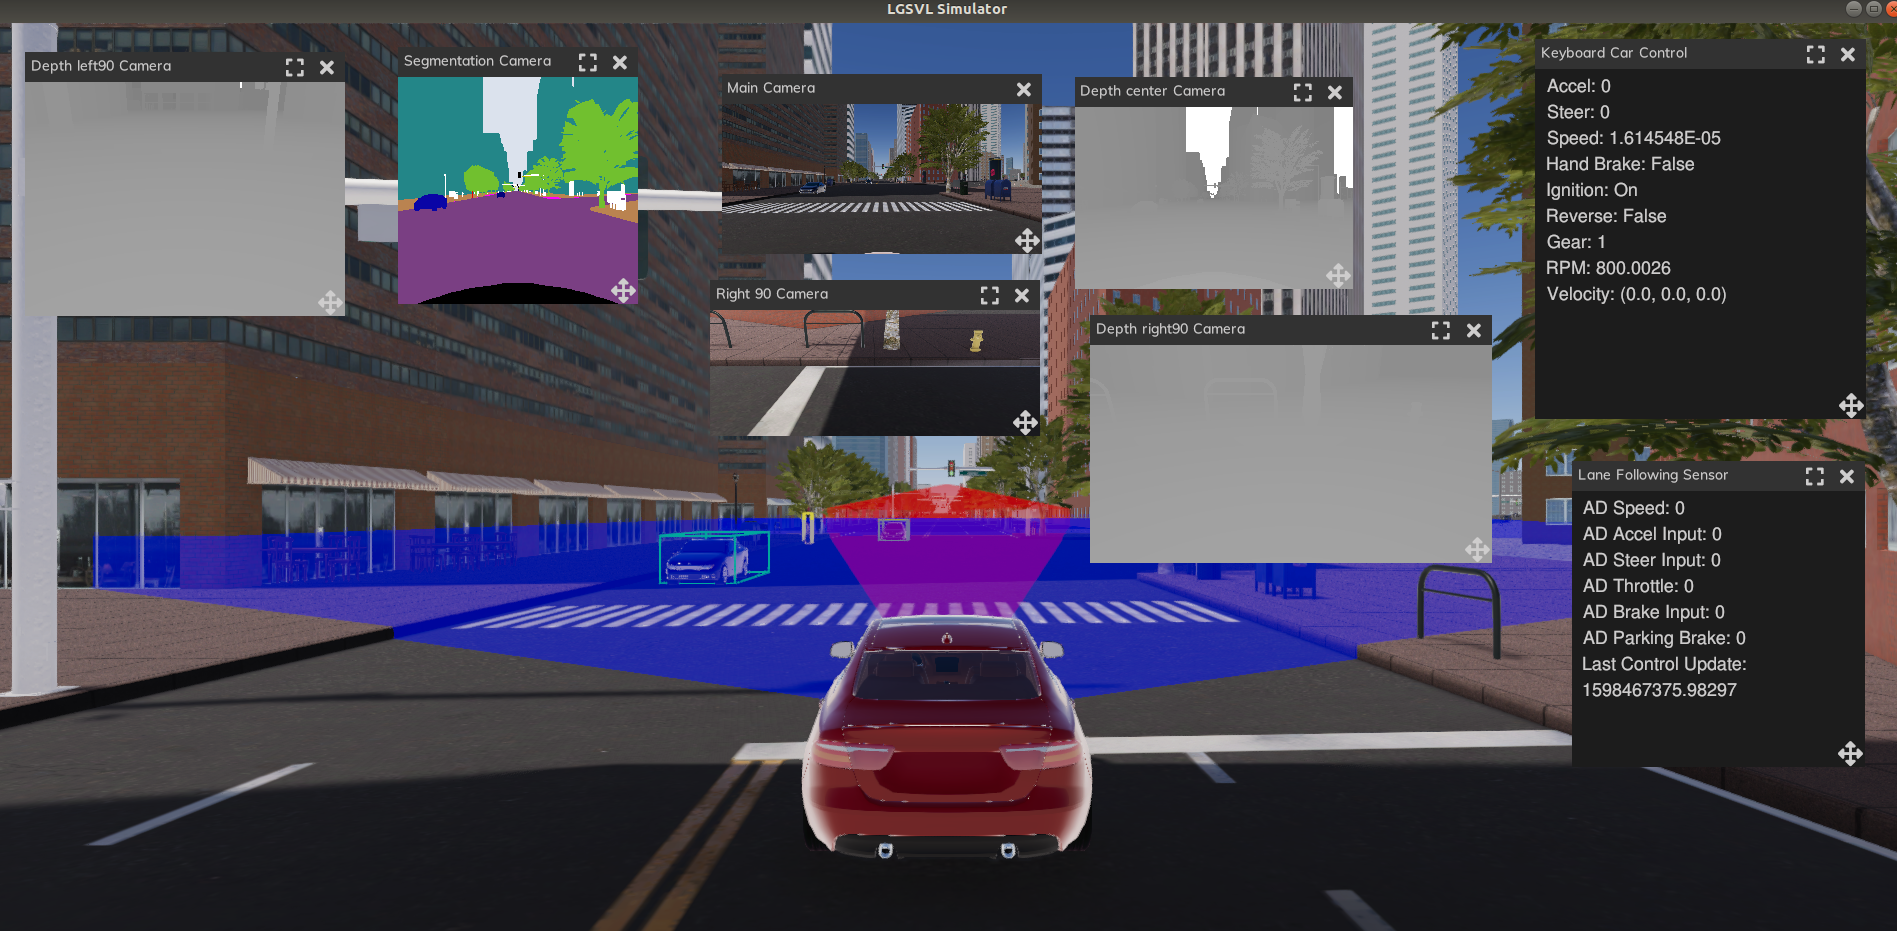
\includegraphics[width = \textwidth]{figures/png/intro/LGSVL_2_scrot_2020-08-26_20-46-55.png}
    \end{center}
    \caption{LGSVL\cite{LGSVL} simulator active with all sensors}
        \label{fig:LGSVL_constellation_sensors}
\end{figure}

%%%%%%%%%%%%%%%
%TODO - 
%insert a table 2.1 in page10 showing how different sensor combo work. Use the thesis under
%reference in firefox.
%https://www.researchgate.net/profile/Markus_Weber14/publication/342283221_Autonomous_Driving_Radar_Sensor_Noise_Filtering_and_Multimodal_Sensor_Fusion_for_Object_Detection_with_Artificial_Neural_Networks/links/5eebe41d458515814a6aa417/Autonomous-Driving-Radar-Sensor-Noise-Filtering-and-Multimodal-Sensor-Fusion-for-Object-Detection-with-Artificial-Neural-Networks.pdf 
%%%%%%%%%%%%%%%%

\section{Goal}
    The desired goals of this thesis are listed below: 

\begin{itemize}
    \item Building an autonomous driving framework -
        \begin{itemize}
        \item ROS - use ROS2 to synchronise the data received from the simulator through a
            rosbrige, use functionalities such as slop and cache, to sort the data according to
            their received time in order not to scramble the information. During the evaluation,
            use the same functionalities to send command controls to the simulator.
        \item Rosbridge - use a bridge transport protocol that connects the ros on the receiving end
            to the simulator on the sending end or vice versa.
        \item Docker - set up a work environment that is independent of hardware or
            operating system which allows easy running of the commands for data collection
            and evaluation.
        \end{itemize}    
    \item Implement an end-to-end neural network architecture which learns to drive by
        training from image pixels to steering commands. Also, apply state of
        the art DL techniques to it.
    \item Implement a system that can efficiently collect and label data.
    \item Implement and analyse different constellation of sensors with different data
        fusion techniques. 
\end{itemize}

\section{Related Work}
In 2012, Alexnet \cite{Alexnet2012} used CNNs to do object classification which, then
in Computer Vision became the dominated approach for classification. Both Chen \textit{et
al.} \cite{chen2017} and Bojarski \textit{et al.} \cite{bojarski2016end} extended
\cite{Alexnet2012}'s approach of using CNN and detailed that in addition to classification, CNN can
extract features from images. Then they went on to demonstrate through an end-to-end
network(which self-optimises itself based on its inputs) steering angles can be predicted that keep the car in the
lane of a road. 

In a different field, but using CNN, Sergey Levine \textit{et al.} 
\cite{GooglePaperonCNNActuation} in 2016 corroborated that it was indeed possible to extract
features with CNN and predict motor control actions in \textit{object picking robots}.

Then, Xu \textit{et al.} \cite{XuGYD16CNNLSTM} in the same year with CNN-LSTM architecture
showed that using the previous ego-motion events helped predict future ego-motion events. 
Using CNNs in an end-to-end architecture raised some questions on how it reached its
decisions. So in 2017, both \cite{heatmapsLearning}, \cite{BojarskiCNN1} did visual
analysis after the CNN layers to better understand the module's functionality. 
Vehicle control is more than just steering control. For smoother control, acceleration and
braking are necessary besides steering. Both acceleration and deacceleration are dependent on  the user's driving
style, lane speed limit and traffic etc. Yand \textit{et
al.} \cite{E2EMultimodalDiscreteSpeed} used CNN-LSTM architecture and provided the LSTM
with feedback speed to determine the velocity of the ego vehicle.

Besides vehicle control, perceiving the environment is necessary for collision avoidance. 
The RGB colour camera sensors don't provide the depth information which is critical for collision avoidance. 
Hence, it is essential to fuse other sensors with diverse modalities with RGB to predict an optimal output. 
Liu \textit{et al.} \cite{liu2018learn} provided rules in fusing data. They said that it was
essential to pick out only vital information and discard other noisy data. 
They also described the techniques involved in data fusion -- early/late
fusion, hybrid fusion, model ensemble and joint training. Park \textit{et
al.} \cite{ParkHBB16} gave us methods to enhance the features by using feature amplification
or multiplicative fusion. Zhou \textit{et al.} \cite{ZhouSideChannel} detailed how fusing
data into CNN affects the overall performance.  

Even though the fused dataset gives a performance boost, it performs worse  
compared to individual modality. The combined fused model overfit more
than its counterparts. The fundamental drawback of
\textit{gradient descent} in backpropagation causes the networks to overfit. This paper \cite{wang2020makes} introduced a technique
called \textit{gradient blending} to counteract this problem.

Xiao \textit{et al.}\cite{XiaoCodevillaMultimodalE2E} applied all the fusion techniques
mentioned above with an imitation based end-to-end network\cite{codevilla2017endtoend}. RGB images with depth information(obtained through a different modality)
could indeed result in better performing end-to-end network model was their conclusion.


\section{Contribution}




